\documentclass[aspectratio=169, 10pt]{beamer}
\usetheme{Madrid}
\usefonttheme{professionalfonts}

\usepackage[english]{babel}
\usepackage[linguistics]{forest}
\usepackage[utf8]{inputenc}
\usepackage{algorithmic}
\usepackage{amsfonts}
\usepackage{amsmath}
\usepackage{amssymb}
\usepackage{array}
\usepackage{bookmark}
% \usepackage{boondox-cal}
\usepackage{caption}
\usepackage{colortbl}
\usepackage{csquotes}
\usepackage{graphicx}
\usepackage{hyperref}
\usepackage{lipsum}
\usepackage{lmodern}
\usepackage{mathptmx}
\usepackage{mathtools}
\usepackage{multirow}
\usepackage{pgfplots}
\usepackage{svg}
\usepackage{xcolor}
\usepackage{tikz}

\newcommand{\vect}{\mathbf}

% \pgfplotsset{compat=1.17}
\usetikzlibrary{calc}

\DeclareMathOperator*{\argmax}{argmax}

\hypersetup{
    colorlinks=true,
    linkcolor=blue,
    filecolor=blue,      
    urlcolor=blue,
}

\title{Tutorial 7}
\subtitle{Tutorial on kNN, SVM, MDP and Q-Learning}
\author{Luke Chang}
\institute{The University of Auckland}
\date{May 2021}


\begin{document}

\frame{\titlepage}

% %-------------------------------------------------------------------------------
\begin{frame}
    \frametitle{Topics}

    \tableofcontents
        
\end{frame}

%-------------------------------------------------------------------------------
\section{Bayesian Networks}
\begin{frame}[t]
    \frametitle{Bayesian Networks}

    \begin{example}
        You are given a toxicity data set that describes chemical compounds with 5 \textit{Boolean}
        attributes water solubility (\textbf{S}), cytochrominhibitor (\textbf{C}), contains phosphate (\textbf{P}), and
        cancerogenic in the rat model (\textbf{R}), and the outcome of some toxicity test (\textbf{O}). For the given
        dataset, could you learn a Bayesian network on the dataset?
    \end{example}
    
    \begin{table}[]
        \small
        \begin{tabular}{cccc|c}
        \textbf{S} & \textbf{C} & \textbf{P} & \textbf{R} & \textbf{O} \\ \hline
        TRUE       & TRUE       & FALSE      & TRUE       & Negative   \\
        TRUE       & FALSE      & TRUE       & TRUE       & Negative   \\
        FALSE      & FALSE      & TRUE       & FALSE      & Negative   \\
        FALSE      & TRUE       & TRUE       & TRUE       & Positive  
        \end{tabular}
    \end{table}

    \vspace{2em}
    If you condition on every attribute (join links top down), \textbf{O} will condition on $4!=24$ possible combinations.
\end{frame}

%-------------------------------------------------------------------------------
\section{Bayesian Networks}
\begin{frame}[t]
    \frametitle{Bayesian Networks}

    \begin{table}[]
        \small
        \begin{tabular}{cccc|c}
        \textbf{S} & \textbf{C} & \textbf{P} & \textbf{R} & \textbf{O} \\ \hline
        TRUE       & TRUE       & FALSE      & TRUE       & Negative   \\
        TRUE       & FALSE      & TRUE       & TRUE       & Negative   \\
        FALSE      & FALSE      & TRUE       & FALSE      & Negative   \\
        FALSE      & TRUE       & TRUE       & TRUE       & Positive  
        \end{tabular}
    \end{table}

    \begin{figure}
        \center
        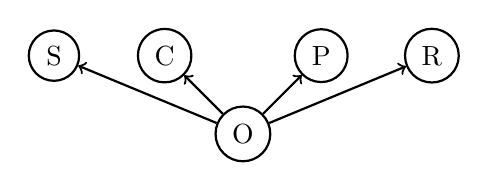
\begin{tikzpicture}[node distance={4em}, thick, main/.style = {draw, circle}] 
            \node[main] (1) {O};
            \node[main] (2) [above left of=1] {C};
            \node[main] (3) [above right of=1] {P};
            \node[main] (4) [left of=2] {S};
            \node[main] (5) [right of=3] {R};

            \draw[<-] (2) -- (1); 
            \draw[<-] (3) -- (1); 
            \draw[<-] (4) -- (1); 
            \draw[<-] (5) -- (1); 
        \end{tikzpicture} 
    \end{figure}

    \begin{table}[]
        \small
        \begin{tabular}{cc}
        P(O) & P($\neg$O) \\ \hline
        0.25 & 0.75 \\
        \end{tabular}
    \end{table}

    \begin{columns}
        \begin{column}{0.25\textwidth}
            \begin{table}[]
                \small
                \begin{tabular}{ccc}
                O & P(S) & P($\neg$S) \\ \hline
                P & 0 & 1.0 \\
                N & 0.666 & 0.333 \\
                \end{tabular}
            \end{table}
        \end{column}
        \begin{column}{0.25\textwidth}
            \begin{table}[]
                \small
                \begin{tabular}{ccc}
                O & P(C) & P($\neg$C) \\ \hline
                P & 1.0 & 0 \\
                N & 0.333 & 0.666 \\
                \end{tabular}
            \end{table}
        \end{column}
        \begin{column}{0.25\textwidth}
            \begin{table}[]
                \small
                \begin{tabular}{ccc}
                O & P(P) & P($\neg$P) \\ \hline
                P & 1.0 & 0.0 \\
                N & 0.666 & 0.333 \\
                \end{tabular}
            \end{table}
        \end{column}
        \begin{column}{0.25\textwidth}
            \begin{table}[]
                \small
                \begin{tabular}{ccc}
                O & P(R) & P($\neg$R) \\ \hline
                P & 1.0 & 0.0 \\
                N & 0.666 & 0.333 \\
                \end{tabular}
            \end{table}
        \end{column}
    \end{columns}

\end{frame}

%-------------------------------------------------------------------------------
\section{Bayesian Networks}
\begin{frame}[t]
    \frametitle{Bayesian Networks}

    \begin{figure}
        \center
        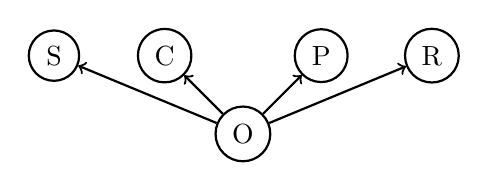
\begin{tikzpicture}[node distance={4em}, thick, main/.style = {draw, circle}] 
            \node[main] (1) {O};
            \node[main] (2) [above left of=1] {C};
            \node[main] (3) [above right of=1] {P};
            \node[main] (4) [left of=2] {S};
            \node[main] (5) [right of=3] {R};

            \draw[<-] (2) -- (1); 
            \draw[<-] (3) -- (1); 
            \draw[<-] (4) -- (1); 
            \draw[<-] (5) -- (1); 
        \end{tikzpicture} 
    \end{figure}

    \begin{table}[]
        \small
        \begin{tabular}{cc}
        P(O) & P($\neg$O) \\ \hline
        \textcolor{red}{0.25} & 0.75 \\
        \end{tabular}
    \end{table}

    \begin{columns}
        \begin{column}{0.25\textwidth}
            \begin{table}[]
                \small
                \begin{tabular}{ccc}
                O & P(S) & P($\neg$S) \\ \hline
                P & \textcolor{red}{0.0} & 1.0 \\
                N & 0.666 & 0.333 \\
                \end{tabular}
            \end{table}
        \end{column}
        \begin{column}{0.25\textwidth}
            \begin{table}[]
                \small
                \begin{tabular}{ccc}
                O & P(C) & P($\neg$C) \\ \hline
                P & 1.0 & \textcolor{red}{0.0} \\
                N & 0.333 & 0.666 \\
                \end{tabular}
            \end{table}
        \end{column}
        \begin{column}{0.25\textwidth}
            \begin{table}[]
                \small
                \begin{tabular}{ccc}
                O & P(P) & P($\neg$P) \\ \hline
                P & 1.0 & \textcolor{red}{0.0} \\
                N & 0.666 & 0.333 \\
                \end{tabular}
            \end{table}
        \end{column}
        \begin{column}{0.25\textwidth}
            \begin{table}[]
                \small
                \begin{tabular}{ccc}
                O & P(R) & P($\neg$R) \\ \hline
                P & 1.0 & \textcolor{red}{0.0} \\
                N & 0.666 & 0.333 \\
                \end{tabular}
            \end{table}
        \end{column}
    \end{columns}

    A new instance with $S=T, C=F, P=F, R=F$, what is the probability of test positive?

    \begin{equation*}
        \begin{array} {rcl}
            P(O=P,S, \neg C, \neg P , \neg F) & = & P(S|O)P(\neg C|O)P(\neg P |O)P(\neg F |O)P(O) \\
            & = & 0.25 \cdot 0.0 \cdot 0.0 \cdot 0.0 = 0.0
        \end{array}
    \end{equation*}

\end{frame}

%-------------------------------------------------------------------------------
\section{K-Nearest Neighbour (kNN) Model}
\begin{frame}[t]
    \frametitle{K-Nearest Neighbour (kNN) Model}

    The k-nearest neighbour fits for $\hat{Y}$ is defined as follows:

    \begin{equation*}
        \hat{Y}(\vect{x}) = \frac{1}{k} \sum_{\vect{x} \in N_k (\vect{x})} y_i
    \end{equation*}

    where $N_k (\vect{x})$ is the neighbourhood of $\vect{x}$ defeined by the $k$ closest 
    points $\vect{x}$ in the training sample.

    \vspace{1em}
    What does kNN do during training?
    \pause
    \begin{itemize}
        \item Saving all training instances
        \item Algorithms used to compute the nearest neighbors:
            \begin{itemize}
                \item Brute-force search
                \item \textbf{KD Tree:} Splits from \textit{median} on every feature; works well in lower dimensional data
                \item \textbf{Ball Tree:} Also a binary tree which partitions data from N-dimensional hyper-sphere; the preferred method for high dimensional data
            \end{itemize}
    \end{itemize}

\end{frame}

%-------------------------------------------------------------------------------
\begin{frame}[t]
    \frametitle{K-Nearest Neighbour (kNN) Model}

    What should you choose for the distance metric?
    \pause
    \begin{itemize}
        \item Euclidean Distance: L$_2$-norm
        \item Manhattan Distance: L$_1$-norm, works better in higher dimensional data
        \item Mahalanobis Distance, Chebyshev Distance (L$_\infty$-norm) and others
    \end{itemize}

    \vspace{1em}
    What are the limitations?
    \pause
    \begin{itemize}
        \item Sensitive to noise
        \item Computational expensive at inference time (Scale by the size of training data)
        \item Does not scale well with larger dataset
    \end{itemize}

\end{frame}

%-------------------------------------------------------------------------------
\section{Support Vector Machine (SVM)}
\begin{frame}[t]
\frametitle{Support Vector Machine (SVM)}


\end{frame}

%-------------------------------------------------------------------------------
\section{Markov Decision Process (MDP)}
\begin{frame}[t]
\frametitle{Markov Decision Process (MDP)}


\end{frame}

%-------------------------------------------------------------------------------
\section{Q-Learning}
\begin{frame}[t]
\frametitle{Q-Learning}


\end{frame}
\end{document}


